%! BibTeX Compiler = biber
%TC:ignore
\documentclass{article}

\usepackage{xcolor, colortbl}
\definecolor{BLUELINK}{HTML}{0645AD}
\definecolor{DARKBLUELINK}{HTML}{0B0080}
\definecolor{LIGHTBLUELINK}{HTML}{3366BB}
\definecolor{PURPLELINK}{HTML}{663366}
\definecolor{RED}{HTML}{EB6231}
\definecolor{GREEN}{HTML}{8FB03E}
\definecolor{LIGHTGREY}{gray}{0.9}
\PassOptionsToPackage{hyphens}{url}
\usepackage[colorlinks=false]{hyperref}
% for linking between references, figures, TOC, etc in the pdf document
\hypersetup{colorlinks,
    linkcolor=DARKBLUELINK,
    anchorcolor=DARKBLUELINK,
    citecolor=DARKBLUELINK,
    filecolor=DARKBLUELINK,
    menucolor=DARKBLUELINK,
    urlcolor=BLUELINK
} % Color citation links in purple
\PassOptionsToPackage{unicode}{hyperref}
\PassOptionsToPackage{naturalnames}{hyperref}

\usepackage{biorxiv}
\usepackage[backend=biber,style=nature]{biblatex}
\addbibresource{codon_models.bib}

\usepackage{url}
\usepackage{amssymb,amsfonts,amsmath,amsthm,mathtools}
\usepackage{textcomp}
\usepackage{gensymb}
\usepackage{cancel}
\usepackage{lmodern}
\usepackage{xfrac, nicefrac}
\usepackage{blkarray}
\usepackage{pgf,tikz}
\usetikzlibrary{positioning,arrows,automata,calc}
\usepackage{bm}
\usepackage{listings, enumerate, enumitem}
\usepackage[export]{adjustbox}
\usepackage{graphicx}
\usepackage{tabu}
\usepackage{hhline}
\usepackage{multicol,multirow,array}
\usepackage{etoolbox}
\usepackage{booktabs}

\usepackage[flushleft] {threeparttable}
\usepackage{bbold}
\usepackage{pdfpages}
\usetikzlibrary{positioning}
\usetikzlibrary{arrows,automata}
\pdfinclusioncopyfonts=1
\usepackage{nicefrac} % compact symbols for 1/2, etc.
\usepackage{microtype} % microtypography
\usepackage{lineno}

\newcommand{\specialcell}[2][c]{%
    \begin{tabular}[#1]{@{}c@{}}
        #2
    \end{tabular}}

\newcommand{\UniDimArray}[1]{\bm{#1}}
\newcommand{\BiDimArray}[1]{\bm{#1}}

\DeclareMathOperator{\E}{\mathbb{E}}
\DeclareMathOperator{\Var}{\mathrm{Var}}
\newcommand{\der}{\mathrm{d}}
\newcommand{\angstrom}{\mathrm{\normalfont\AA}}
\newcommand{\e}{\mathrm{e}}
\newcommand{\avg}[1]{\left< #1 \right>} % for average
\newcommand{\Ne}{N_{\mathrm{e}}}
\newcommand{\Ner}{N_{\mathrm{r}}}
\newcommand{\dn}{d_N}
\newcommand{\ds}{d_S}
\newcommand{\dnds}{\dn / \ds}
\newcommand{\pn}{\pi_N}
\newcommand{\ps}{\pi_S}
\newcommand{\pnps}{\pn / \ps}
\newcommand{\proba}{\mathbb{P}}
\newcommand{\pfix}{\proba_{\mathrm{fix}}}
\newcommand{\Pfix}{2 \Ne \proba_{\mathrm{fix}}}
\newcommand{\indice}{a}
\newcommand{\indiceexp}{^{(\indice)}}

\renewcommand{\baselinestretch}{1.5}
\renewcommand{\arraystretch}{0.6}
\linenumbers

\title{Selection coefficients at the phylogenetic and population-genetic scale}

\author{
    \large
    T. {Latrille}$^{1}$, J. {Joseph}$^{2}$, N. {Salamin}$^{1}$\\
    $^{1}$Université de Lausanne, Lausanne, Switzerland
    $^{1}$Université de Lyon, Lyon, France
}

\begin{document}
    \maketitle

    \begin{abstract}
        At the phylogenetic scale, recent mutation-selection models provide a direct estimate of the selection coefficient for any mutation in a coding sequence, depending on the amino-acids involved in the mutation.
        At the population-genetic scale, the frequency at which a polymorphism segregates in a population is also a function of its selection coefficient.
        Taking advantage of this relationship between phylogenetic and population genetics, we can assess whether selection coefficients estimated at the phylogenetic scale can predict the frequency of polymorphism.
        In this study, we integrated divergence and polymorphism data across the entire exome for 29 populations across 7 genera, and showed that selection coefficients are correlated at the phylogenetic and population-genetic scales.
        Altogether, our work is paving the way for studies and methods augmenting molecular polymorphism data within species with information about divergence data between species, and by assessing empirically the relationship between phylogenetic and population genetics.
    \end{abstract}

    \keywords{Selection \and phylogenetic \and population genetics \and codon models}

    \tableofcontents

    \section{Introduction}\label{sec:introduction}
%TC:endignore

    In phylogeny-based methods, mutation-selection models provide a nearly-neutral model of evolution by estimating the fitness landscape over amino-acid sequences, for each site of the sequence\cite{yang_mutationselection_2008, halpern_evolutionary_1998, rodrigue_mechanistic_2010}.
    At the mutation-selection balance, the probability for a specific codon to be fixed in the population is proportional to its fitness, and a mutation from a high fitness amino-acid towards a low fitness amino-acid will have a small probability of fixation, genuinely accounting for purifying selection.
    Conversely, only nearly-neutral mutations between high fitness amino acids will tend to be permitted by the model, allowing for the explicit calculation of the scaled selection coefficient of non-synonymous mutations at mutation-selection balance\cite{spielman_relationship_2015, rodrigue_detecting_2017}.
    In this study, we thus first applied mutation-selection codon models to whole exome data from placental mammals, such as to quantify the amino-acid fitness profile for each site of each protein.

    The goal of this study is to assess whether the signal of selection at the phylogenetic and population-genetic scale are correlated.
    The population- and phylogeny-based methods work over very different time scales, for that reason, they might be capturing different signals.
    Nonetheless, we expect sites and proteins under long-term evolution to maintain their signal of selection in several independent lineages for which we computed the unfolded site frequency spectrum (SFS).
    To test this hypothesis, we leverage a pipeline integrating divergence and polymorphism data across the entire exome for 29 populations across 7 genera, namely \textit{Equus}, \textit{Canis}, \textit{Bos}, \textit{Capra}, \textit{Ovis}, \textit{Chlorocebus} and \textit{Homo}.

%TC:ignore


    \section{Methods}\label{sec:methods}

    \subsection*{Phylogenetic dataset}
    protein-coding DNA sequences alignments in placental mammals are extracted from the \href{https://www.orthomam.univ-montp2.fr}{OrthoMaM} database\cite{ranwez_orthomam_2007, douzery_orthomam_2014, scornavacca_orthomam_2019}.
    Genes located on the X, Y and mitochondrial chromosome are discarded from the analysis, since the number of polymorphism, necessary in population-based method, is expected to be different on these sequences.
    Additionally, sequences from the species for which polymorphism are available, as well as their sister species have been discarded from the analysis to ensure independence between the data used in the phylogenetic and population-genetic method.

    \subsection{Selection coefficient in phylogeny-based method}
    Mutation-selection models assume that the protein-coding sequence is at mutation-selection balance under a fixed fitness landscape, which is itself characterized by a fitness vector over the $20$ amino-acid at each site\cite{yang_mutationselection_2008, halpern_evolutionary_1998, rodrigue_mechanistic_2010}.
    Mathematically, the rate of non-synonymous substitution from codon $a$ to codon $b$ ($q_{a \mapsto b}^{(i)}$) at site $i$ of the sequence is equal to the rate of mutation from the underlying DNA change ($\mu_{a \mapsto b}$) multiplied by the scaled probability of fixation of the mutation ($\proba_{a \mapsto b}^{(i)}$).
    Crucially, the probability of fixation depends on the difference of scaled fitness between the amino-acid encoded by the mutated codon ($F_b^{(i)}$) and the fitness of the amino-acid encoded by the original codon ($F_a^{(i)}$) of site $i$\cite{wright_evolution_1931, fisher_genetical_1930}.
    Altogether, the rate of substitution from codon $a$ to $b$ at a given site $i$ is:
    \begin{equation}
        q_{a \mapsto b}^{(i)} = \mu_{a \mapsto b} \proba_{a \mapsto b}^{(i)} = \mu_{a \mapsto b} \dfrac{F_b^{(i)} - F_a^{(i)}}{1 - \e^{F_a^{(i)} - F_b^{(i)}}}.
    \end{equation}

    Fitting the mutation-selection model on a sequence alignment leads to an estimation of the mutation rate matrix ($\UniDimArray{\mu}$) as well as the 20 amino-acid fitness landscape ($\UniDimArray{F^{(i)}}$) at each site $i$.

    We ran the Bayesian software \href{https://github.com/bayesiancook/bayescode}{BayesCode} on each protein-coding DNA alignment\cite{lartillot_phylobayes_2013, rodrigue_detecting_2017}.
    Each Monte-Carlo Markov-Chain (MCMC) is run during $2000$ points, with a burn-in of $1000$ points, allowing to compute the mean amino-acid fitness landscape ($\UniDimArray{F^{(i)}}$) at each site $i$ across the MCMC.

    \subsection{Polymorphism dataset}

    In order to compare polymorphism and divergence, each SNP (chromosome, position, strand) in the focal species must be matched to its relative position in the protein-coding DNA alignment.
    First, genomic positions are converted to relative position in the coding sequence (CDS) using gene annotation files (GTF format) downloaded from Ensembl (\url{ensembl.org}), we verified the SNP match the reference in the CDS (FASTA format) also downloaded from Ensembl.
    Secondly, relative position in the CDS is converted to position in the multiple sequence alignment (containing gaps) from OrthoMaM database\cite{ranwez_orthomam_2007, douzery_orthomam_2014, scornavacca_orthomam_2019} by doing a global pairwise alignment (Biopython pairwise2) between the CDS fasta and the sequence found in the alignment.
    This conversion from genomic position to position in the alignment is only possible if the assembly used for SNP calling is the same as the one used in the alignment, the GTF annotations and the FASTA sequences.
    We retrieved polymorphism from different projects.
    \textit{Equus caballus} variants called on the EquCab2 assembly in the EVA study PRJEB9799, we considered \textit{Ceratotherium simum simum} as its sister species.
    \textit{Canis familiars} variants called on the CanFam3.1 assembly in the EVA study PRJEB24066, we considered \textit{Ursus maritimus} as its sister species.
    \textit{Bos taurus} variants called on the UMD3.1 assembly in the next-gen project, we considered \textit{Bison bison bison} as its sister species.
    \textit{Ovis aries} variants called on the Oar\_v3.1 assembly in the next-gen project, we considered \textit{Pantholops hodgsonii} as its sister species.
    \textit{Capra Hircus} variants called on the CHIR1 assembly in the next-gen project, we performed a liftover to the ARS1 assembly and considered \textit{Pantholops hodgsonii} as its sister species.
    \textit{Chlorocebus sabaeus} variants are called on the ChlSab1.1 assembly in the EVA study PRJEB22989\cite{svardal_ancient_2017}, we considered \textit{Macaca mulatta} as its sister species.
    \textit{Homo sapiens} variants are called on the GRCh38 assembly in the 1000-genome project\cite{consortium_integrated_2012, the1000genomesprojectconsortium_global_2015}, we considered \textit{Pan troglodytes} as its sister species.
    Variants not inside genes are discarded at the beginning of the analysis.
    Insertions and deletions are not analyzed, and only Single Nucleotide Polymorphisms (SNPs) with only one mutant allele are considered.
    Stop codon mutants are also discarded.
    For populations containing more than $8$ sampled individuals, the site-frequency spectrum (SFS) is subsampled down to $16$ chromosomes ($8$ diploid individuals) without replacement (hyper-geometric distribution) to alleviate the effect of different sampling depth in the $29$ populations.
    Moreover, subsampling mitigate the impact of moderately deleterious mutations segregating at low frequency on $\pnps$, since they are more likely to be discarded than polymorphism segregating at higher frequency.
    SNPs are polarized using the $3$ closest outgroups found in the OrthoMam alignment with est-usfs\cite{keightley_inferring_2018}.
    The Snakemake pipeline for integrating polymorphism and divergence data uses custom scripts written in python 3.8.

    \subsection{Site frequency spectrum}
    The probability of fixation of an allele can be empirically observable, and in the context of a Wright-Fisher processes it is related to selection and drift.
    However, this absorbing fate is not the sole characteristic of the process that relates empirical observable quantities to parameters of the process.
    Along the whole trajectory of an allele, before fixation or extinction, the probability of this allele to be at a certain frequency can be related to its selection coefficient and to the effective population size.
    More precisely, $g(x) \der x $ is the expected time for which the population frequency of derived allele is in the range $(x, x+\der x)$ before eventual absorption, which is derived using the Kolmogorov forward equation as a function of $x$ and $S$:
    \begin{align}
        g(x, s, \Ne) & = \dfrac{\left( 1 - \e^{- 2 s }\right) \left( 1 - \e^{-4 \Ne s(1-x)}\right)}{ s (1 - \e^{-4 \Ne s})x(1-x)} \\
        \Rightarrow g(x, S) & \approx \dfrac{2 \left( 1 - \e^{-S(1-x)}\right)}{(1 - \e^{-S})x(1-x)} \label{eq:expected_time}
    \end{align}

    \begin{center}
        \includegraphics[width=0.4\textwidth, page=4] {artworks/figures.pdf}
        \flushleft
        Expected time at a derived frequency $g(x, S)$ in the vertical axis as a function of the frequency $x$, shown for different scaled selection coefficient.
        Allele with a positive selection coefficient can be observed at high frequency, while alleles with negative selection coefficients are unlikely to be observed at high frequency.
    \end{center}

    This equation is solely valid for a gene with two alleles, a configuration which is rarely observed in empirical data since more than two variants of a gene are usually present in the population.
    However, it is frequent to observe sites inside a gene sequence for which only two alleles are segregating.
    This observation led to the development of a site-specific Wright-Fisher process, assuming that each site follows an independent process.
    Strictly speaking, this model considers a collection of independently evolving loci, meaning without linkage.
    It provides a good approximation if there is free recombination between sites.
    Moreover, the collection is considered infinite whereas the total mutation rate across this infinite collection is considered finite.
    The assumption of an infinite number of sites is necessary to ensure that each mutation arises at a new site, with a Poisson distribution of total rate $u$ per generation for the whole sequence.

    From an empirical perspective, for a sample of $n$ sequences taken in the population, the expected number of sites with $i$ copies of the derived allele (with $i$ ranging from $1$ to $n - 1$) is denoted $G(i, n)$.
    The collection of all $G(i, n)$ generates what is called a site frequency spectrum ({SFS}), which can intuitively be interpreted as the discrete version of the expected time at a derived frequency, readily available from a sample of sequences from a population.
    Given the scaled selection coefficient ($S=4 \Ne s$), and the scaled mutation rate per generation for the whole sequence ($\theta = 4 \Ne u $), each entry of the {SFS} is:
    \begin{align}
        G(i, n) & = \int_{0}^{1}  2 \Ne u g(x, S) \binom{n}{i} x^{i} (1-x)^{n-i} \der x \\
        & = \theta \int_{0}^{1} \dfrac{1 - \e^{-S(1-x)}}{(1 - \e^{-S})x(1-x)} \binom{n}{i} x^{i} (1-x)^{n-i} \der x \\
        & =  \dfrac{\theta }{1 - \e^{-S}} \binom{n}{i} \int_{0}^{1} \left( 1 - \e^{-S(1-x)} \right) x^{i-1} (1-x)^{n-i-1} \der x
    \end{align}

    This site frequency spectrum can be confronted to empirical polymorphic data in order to estimate the scaled selection coefficient of new mutations.
    However, a single selection coefficient for all sites and all mutations is biologically not realistic.
    Accordingly, a distribution of selection coefficients across sites is assumed, which is usually modelled as a continuous distribution, known as the distribution of fitness effects of mutations (DFE).
    Mixing over this distribution, the SFS can then be computed as a function of the underlying DFE, and can thus be estimated based on empirical data\cite{eyre-walker_distribution_2006, eyre-walker_estimating_2009}.

    \printbibliography
\end{document}